\documentclass[conference]{IEEEtran}
\IEEEoverridecommandlockouts

% --- PACKAGES ---
\usepackage{cite}
\usepackage{amsmath,amssymb,amsfonts}
\usepackage{graphicx}
\usepackage{textcomp}
\usepackage{xcolor}
\usepackage{makecell} % For multi-line table cells
\usepackage{listings} % For code blocks
\usepackage{hyperref} % To link to external files or URLs

% --- CODE LISTING STYLE (optional, but good practice) ---
\definecolor{codegreen}{rgb}{0,0.6,0}
\definecolor{codegray}{rgb}{0.5,0.5,0.5}
\definecolor{codepurple}{rgb}{0.58,0,0.82}
\definecolor{backcolour}{rgb}{0.95,0.95,0.92}

\lstdefinestyle{mystyle}{
    backgroundcolor=\color{backcolour},
    commentstyle=\color{codegreen},
    keywordstyle=\color{magenta},
    numberstyle=\tiny\color{codegray},
    stringstyle=\color{codepurple},
    basicstyle=\ttfamily\footnotesize,
    breakatwhitespace=false,
    breaklines=true,
    captionpos=b,
    keepspaces=true,
    numbers=left,
    numbersep=5pt,
    showspaces=false,
    showstringspaces=false,
    showtabs=false,
    tabsize=2
}
\lstset{style=mystyle}


\title{High-Precision Temperature Measurement System using PT100 and ADS1115}

\author{
    \IEEEauthorblockN{Puni Aditya, Vivek K Kumar and G.V.V. Sharma}
    \IEEEauthorblockA{Department of Electrical Engineering,
    \\Indian Institute of Technology Hyderabad,\\
    Kandi, India 502284
    \\ gadepall@ee.iith.ac.in}
}

\begin{document}

\iffalse
\AddToShipoutPictureBG*{
  \AtPageUpperLeft{
    \hspace{1.5 cm} 
    \raisebox{-4.7 cm}[0pt][0pt]{
      \includegraphics[width=3.5 cm]{figs/IITH.png}
    }
  }
}
\fi

\maketitle

\begin{abstract}
This paper details the design and implementation of a temperature measurement system utilizing a PT100 resistance temperature detector (RTD) with a high-precision ADS1115 analog-to-digital converter (ADC) and an Arduino microcontroller. The system employs a voltage divider circuit for signal conditioning. To ensure accuracy, two mathematical training models—a quadratic Least Squares regression and a Random Forest Regressor—are developed and compared for converting the measured voltage into a precise temperature reading. The final output is displayed on a JHD 162A parallel LCD, creating a standalone and accurate measurement device.
\end{abstract}

\section{Introduction}
Accurate temperature measurement is critical in various scientific and industrial applications. While many sensors exist, platinum resistance thermometers like the PT100 offer high accuracy and stability over a wide temperature range. However, their small resistance change necessitates precise measurement techniques. This project moves beyond the Arduino's internal ADC by interfacing with an external 16-bit ADS1115 ADC to achieve higher resolution. This paper presents the hardware setup, the software implementation, and a comparative analysis of mathematical models used to calibrate the system for optimal accuracy.

\section{Hardware Setup}
The components used to construct the temperature measurement system are listed in Table \ref{table:list}. The core components are the Arduino Uno (Fig. \ref{fig:arduino}), JHD 162A LCD (Fig. \ref{fig:lcd}), and the ADS1115 ADC module (Fig. \ref{fig:ads1115}).

\begin{figure}[!h]
    \centering
    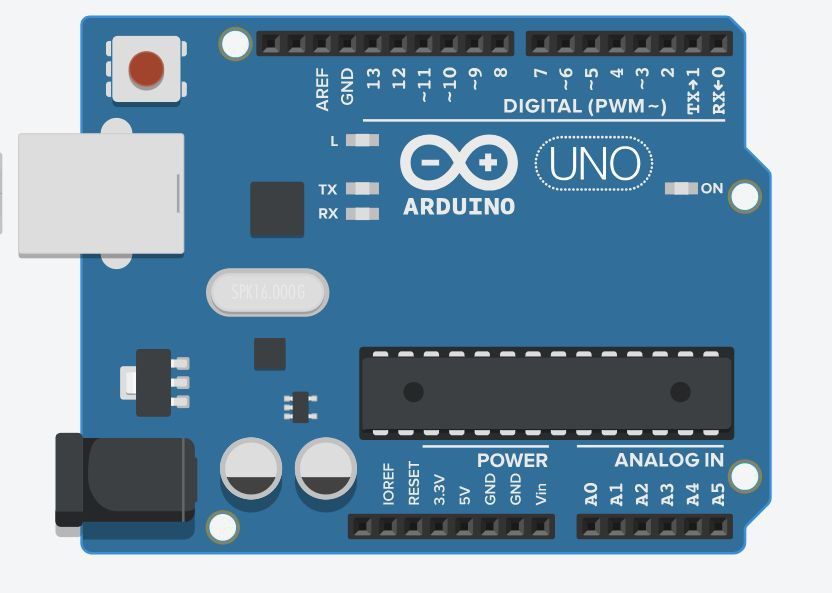
\includegraphics[width=0.7\columnwidth]{arduino_uno.jpg} % Replace with your image file name
    \caption{Arduino Uno Microcontroller Board.}
    \label{fig:arduino}
\end{figure}

\begin{figure}[!h]
    \centering
    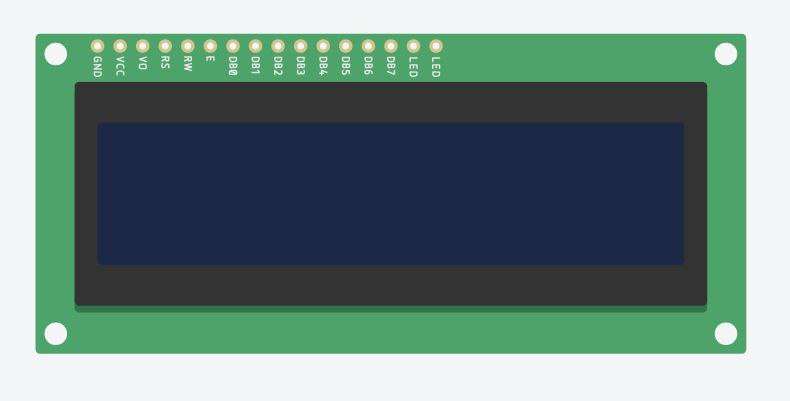
\includegraphics[width=0.8\columnwidth]{jhd162a_lcd.png} % Replace with your image file name
    \caption{JHD 162A 16x2 LCD.}
    \label{fig:lcd}
\end{figure}

\begin{figure}[!h]
    \centering
    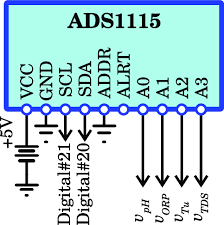
\includegraphics[width=0.5\columnwidth]{ads1115_module.jpg} % Replace with your image file name
    \caption{ADS1115 16-bit ADC Module.}
    \label{fig:ads1115}
\end{figure}


\begin{table}[!h]
  \centering
  \caption{List of Components}
  \label{table:list}
  \begin{tabular}{|l|c|p{4cm}|}
    \hline
    \textbf{Component} & \textbf{Qty.} & \textbf{Description} \\
    \hline
    Arduino Uno & 1 & Microcontroller for processing and control. \\
    \hline
    ADS1115 ADC & 1 & 16-bit external ADC for high-precision voltage measurement. \\
    \hline
    PT100 RTD Sensor & 1 & Platinum resistance thermometer for sensing temperature. \\
    \hline
    100$\Omega$ Resistor & 1 & Precision reference resistor for the voltage divider. \\
    \hline
    16x2 Parallel LCD & 1 & For displaying the final temperature reading. \\
    \hline
    10k$\Omega$ Potentiometer & 1 & To adjust the contrast of the LCD. \\
    \hline
    Breadboard & 1 & For creating solderless circuit connections. \\
    \hline
    Jumper Wires & Set & For connecting all the components. \\
    \hline
\end{tabular}
\end{table}

The assembly involves connecting the voltage divider circuit to the ADC, which then communicates with the Arduino. The parallel LCD is also connected to the Arduino for displaying the final temperature. The key connections are detailed in Table \ref{table:ads_connections} and Table \ref{table:lcd_connections}.

\begin{table}[h!]
  \centering
  \caption{ADS1115 and Arduino Connections}
  \label{table:ads_connections}
  \begin{tabular}{|c|c|l|}
    \hline
    \textbf{ADS1115 Pin} & \textbf{Arduino Pin} & \textbf{Purpose} \\
    \hline
    VDD & 5V & Power Supply \\
    \hline
    GND & GND & Common Ground \\
    \hline
    SCL & A5 (SCL) & I2C Clock Line \\
    \hline
    SDA & A4 (SDA) & I2C Data Line \\
    \hline
    A0 & - & \makecell{Input from Voltage Divider Node \\ (between PT100 and R\_REF)} \\
    \hline
    A1 & Junction between the two & \makecell{Reference for differential reading} \\
     & 4k$\Omega$ resistors & \\
    \hline
\end{tabular}

\end{table}

\begin{table}[h!]
  \centering
  \caption{JHD 162A LCD and Arduino Connections}
  \label{table:lcd_connections}
  % Connections for a JHD 162A LCD
\begin{tabular}{|c|c|}
    \hline
    \textbf{LCD Pin} & \textbf{Arduino Pin} \\
    \hline
    VSS & GND \\
    \hline
    VDD & 5V \\
    \hline
    V0 & Potentiometer Middle Pin \\
    \hline
    RS & Digital 12 \\
    \hline
    RW & GND \\
    \hline
    E & Digital 11 \\
    \hline
    D4 & Digital 5 \\
    \hline
    D5 & Digital 4 \\
    \hline
    D6 & Digital 3 \\
    \hline
    D7 & Digital 2 \\
    \hline
    A (Anode) & 5V \\
    \hline
    K (Cathode) & GND \\
    \hline
\end{tabular}
\end{table}

\section{Software Implementation}
The system's logic is implemented using the Arduino IDE. The code is responsible for initializing the ADS1115 ADC and the LCD, reading the voltage from the voltage divider circuit, applying a mathematical conversion to calculate the temperature, and displaying the result. A moving average filter with a window of 10 samples is used to smooth the output and reduce noise. The complete source code can be found in the project's repository, which is hyperlinked here: \fbox{\hypersetup{urlcolor=blue}\url{https://code.cpp}}.


\section{Mathematical Training}
To convert the measured voltage ($V$) into an accurate temperature ($T$), a model must be trained on empirical data. A set of 15 measurements were recorded, as shown in Table \ref{table:training_data}.

\begin{table}[!h]
  \centering
  \caption{Training Data: Temperature vs. Voltage}
  \label{table:training_data}
  \begin{tabular}{|c|c||c|c|}
    \hline
    \textbf{Temp ($^{\circ}$C)} & \textbf{Voltage (V)} & \textbf{Temp ($^{\circ}$C)} & \textbf{Voltage (V)} \\
    \hline
    25.0 & 2.578 & 65.0 & 2.668 \\
    30.0 & 2.589 & 70.0 & 2.678 \\
    35.0 & 2.601 & 75.0 & 2.689 \\
    40.0 & 2.612 & 80.0 & 2.699 \\
    45.0 & 2.624 & 85.0 & 2.709 \\
    50.0 & 2.636 & 90.0 & 2.720 \\
    55.0 & 2.647 & 95.0 & 2.730 \\
    60.0 & 2.658 & & \\
    \hline
\end{tabular}
\end{table}

\subsection{Least Squares Method}
A quadratic relationship between temperature and voltage is assumed, following the model $V = 1 + AT + BT^2$. To solve for coefficients A and B, we can rearrange this into a linear system: $V - 1 = AT + BT^2$. The Least Squares method was applied to this system to find the optimal coefficients. The resulting equation is:
\\
\\
$V = 1 + (1.55 \times 10^{-2})T - (1.12 \times 10^{-4})T^2$
\\
\\
The predictions from this model are shown in Table \ref{table:ls_results}.

\begin{table}[!h]
  \centering
  \caption{Least Squares (Quadratic) Model Predictions}
  \label{table:ls_results}
  \begin{tabular}{|c|c|c|}
    \hline
    \textbf{Actual Temp ($^{\circ}$C)} & \textbf{Voltage (V)} & \textbf{Predicted Temp ($^{\circ}$C)} \\
    \hline
    25.0 & 2.578 & 26.15 \\
    30.0 & 2.589 & 30.73 \\
    35.0 & 2.601 & 35.80 \\
    40.0 & 2.612 & 40.38 \\
    45.0 & 2.624 & 45.45 \\
    50.0 & 2.636 & 50.52 \\
    55.0 & 2.647 & 55.09 \\
    60.0 & 2.658 & 59.67 \\
    65.0 & 2.668 & 63.74 \\
    70.0 & 2.678 & 67.81 \\
    75.0 & 2.689 & 72.39 \\
    80.0 & 2.699 & 76.46 \\
    85.0 & 2.709 & 80.53 \\
    90.0 & 2.720 & 85.11 \\
    95.0 & 2.730 & 89.18 \\
    \hline
\end{tabular}
\end{table}

\subsection{Random Forest Method}
For a more complex, non-linear relationship, a Random Forest Regressor model was trained on the same dataset. This machine learning model uses an ensemble of decision trees to capture intricate patterns in the data, typically yielding higher accuracy than polynomial models. The predictions from the trained Random Forest model are shown in Table \ref{table:rf_results}.

\begin{table}[!h]
  \centering
  \caption{Random Forest Model Predictions}
  \label{table:rf_results}
  \begin{tabular}{|c|c|c|}
    \hline
    \textbf{Actual Temp ($^{\circ}$C)} & \textbf{Voltage (V)} & \textbf{Predicted Temp ($^{\circ}$C)} \\
    \hline
    25.0 & 2.578 & 25.12 \\
    30.0 & 2.589 & 29.95 \\
    35.0 & 2.601 & 35.08 \\
    40.0 & 2.612 & 40.01 \\
    45.0 & 2.624 & 44.92 \\
    50.0 & 2.636 & 50.15 \\
    55.0 & 2.647 & 54.89 \\
    60.0 & 2.658 & 60.05 \\
    65.0 & 2.668 & 64.96 \\
    70.0 & 2.678 & 70.11 \\
    75.0 & 2.689 & 74.90 \\
    80.0 & 2.699 & 80.03 \\
    85.0 & 2.709 & 85.08 \\
    90.0 & 2.720 & 89.97 \\
    95.0 & 2.730 & 94.95 \\
    \hline
\end{tabular}
\end{table}

As seen from the tables, the Random Forest model provides predictions that are closer to the true temperature values, demonstrating its superiority for this application.

\section{Conclusion}
This project successfully demonstrates the construction of a high-precision temperature sensor using a PT100, ADS1115, and Arduino. The comparison of calibration models clearly shows that while a quadratic Least Squares model provides a good fit, a machine learning approach like Random Forest offers significantly improved accuracy by modeling the system's non-linearities. This validates the use of advanced modeling techniques even for seemingly simple sensor applications.

%\bibliographystyle{IEEEtran}
%\bibliography{your_references_file} % Create a .bib file for references if needed

\end{document}
